\documentclass{sig-alternate}

\usepackage[usenames, dvipsnames]{color}
\usepackage{times}
\usepackage{xspace}
\usepackage{textcomp}
\usepackage{wrapfig}
\usepackage{graphicx}
\usepackage{url}
%\usepackage{amsmath, amssymb}
\usepackage[protrusion=true,expansion=true]{microtype}
\usepackage{comment}
\usepackage{alltt}
\usepackage{appendix}
%\usepackage{algorithm}
%\usepackage{algorithmic}
\usepackage{booktabs}
\usepackage{color}
\usepackage{listings}
\lstset{ %
basicstyle=\ttfamily\scriptsize,       % the size of the fonts that are used for the code
numbers=left,                   % where to put the line-numbers
numberstyle=\ttfamily,      % the size of the fonts that are used for the line-numbers
%aboveskip=0pt,
%belowskip=0pt,
stepnumber=1,                   % the step between two line-numbers. If it is 1 each line will be numbered
%numbersep=10pt,                  % how far the line-numbers are from the code
breakindent=0pt,
firstnumber=0,
%backgroundcolor=\color{white},  % choose the background color. You must add \usepackage{color}
showspaces=false,               % show spaces adding particular underscores
showstringspaces=false,         % underline spaces within strings
showtabs=false,                 % show tabs within strings adding particular underscores
frame=leftline,
tabsize=2,  		% sets default tabsize to 2 spaces
captionpos=b,   		% sets the caption-position to bottom
breaklines=false,    	% sets automatic line breaking
breakatwhitespace=true,    % sets if automatic breaks should only happen at whitespace
%escapeinside={\%}{)}          % if you want to add a comment within your code
columns=fixed,
basewidth=0.52em,
% are you fucking kidding me lstlistings?  who puts the line numbers outside the margin?
xleftmargin=6mm,
xrightmargin=-6mm,
numberblanklines=false,
language=Ruby,
morekeywords={declare,table,scratch,channel,interface,periodic}
}
\lstset{escapeinside={(*}{*)}}
%\renewcommand*\thelstnumber{\the\value{lstnumber}:}


%\linespread{0.975}

\newcommand{\jmh}[1]{{\textcolor{red}{#1 -- jmh}}}
\newcommand{\paa}[1]{{\textcolor{blue}{#1 -- paa}}}
\newcommand{\pb}[1]{{\textcolor{green}{#1 -- kc}}}
\newcommand{\smallurl}[1]{{\small \url{#1}}}

\begin{document}
\title{CALM and Safe: Understanding When Computers Should Coordinate}

\numberofauthors{1}
\author{
Authors
}

\maketitle

\begin{abstract}
We present a foundation for applied researchers to understand recent research on the role of coordination in computer systems.  We discuss the mechanism-independent essence of coordination, and illustrate how technology trends make coordination increasingly problematic in modern systems at many scales.  We describe the CALM Theorem~\cite{}, a foundation for capturing precisely when coordination is needed and when it can be avoided.  Earlier treatments of the theorem covered properties of program end-states (``liveness''); we show how the theorem can also be used to assess invariant properties during execution (``safety'').  Finally, we discuss design patterns that have emerged for avoiding coordination in this context.  
\end{abstract}

\section{Introduction}
There has been substantial research in recent years on the computational role of \emph{coordination}: techniques that are used to enforce order among cooperating processes.  The design of mechanisms to achieve coordination goes back to the earliest days of computer and database systems~\cite{grayreuter,seminalosbook}, including shared-memory mechanisms like semaphores~\cite{semaphores} and locks~\cite{2pl}, and message passing protocols for commit~\cite{2pl,3pl} and consensus~\cite{paxos,virtualsynchrony}.  An enormous variety of variations and enhancements to these techniques have been developed over the decades since these issues were first codified.

The advances of Moore's Law and the attendant rise of global-scale computing has led to a situation where coordination protocols are a significant bottleneck at all levels of the memory hierarchy; we explore this topic in detail in Section~\ref{sec:costs}.  As a result of the painful cost...


\subsection{Contributions of This Paper}
\begin{itemize}
\item We describe coordination in a mechanism-independent fashion, and examine the motivation for its use in concurrent and distributed programs.
\item We provide a trend analysis of the cost of coordination across multiple scales, showing that it is one of the most significant performance \jmh{latency?  tput?  goodput?} problems in modern computing, and will only grow more significant.
\item We present a practitioner's decription of the CALM theorem, including detailed discussion of its assumptions, intuition about its correctness, and discussion of its applicability in analyzing and writing distributed software.
\item We unify the CALM Theorem with a later result in this space: the notion of Invariant Confluence~\cite{}.  
\item We discuss recent design patterns including CRDTs~\cite{crdts} and more extended lattice APIs~\cite{blooml} in the context of CALM.
\end{itemize}

\section{What is Coordination?}
Regardless of the language or model of computation, even sequential software inherently involves some kind of ``waiting''.  But coordination is a particular kind of waiting used in concurrent programming.  Before we ask the question of when coordination is necessary, we must carefully distinguish coordination from other forms of waiting that arise in a sequential context.

Consider a simple sequential program that includes a statement $s$ that computes $x + y$.  To execute $s$, we must first know the values of variables---$x$ and $y$ must be ``instantiated''.  These values may need to be computed by other statements, and/or acquired from relatively slow or asynchronous sources (e.g., off-cache memory, I/O devices, remote computers, or user input).  Waiting for these variables to be instantiated is a requirement of the program's specification, captured as \emph{data dependencies}.  These do not change in a concurrent setting.  Moreover, this waiting cost of data dependencies can often be mitigated or eliminated by intelligent data placement---this is the essence of techniques like caching, prefetching, distributed data placement, etc.  Data dependency delays are \emph{not} the result of a need for coordination, and they do not require or benefit from the use of coordination protocols like semaphores, locks, commit or consensus protocols.  Hence we want to define coordination in a way that distinguishes it carefully from data dependencies.

\emph{Need a simplified model of a single process participating in a concurrent execution: probably just a sequence of operations.  Then talk about ``enhancing'' this process with additional coordination code that is embedded into this sequence.  Push aside the question of analyzing a program to see if it's ``coordinating''.}

We say that a process engages in \emph{coordination} when:
\begin{enumerate}
\item All of the variables required for the process to execute step $s$ are instantiated.
\item Prior to executing step $s$, the process invokes its coordination logic.
\item The coordination logic chooses to wait for a signal from another process.
\end{enumerate}

\emph{a little diagram here would be nice: original sequential thread; thread ``broken'' into to with coord stuck in the middle, spinning, even though the ``second half'' of the thread is ready to go.  need some visual for ``ready to go''}

Note how the first step of this definition distinguishes coordination from data dependencies.  A coordination-free program allows data to ``flow'' freely, and processes are free to proceed as soon as they have the data they need.  The role of coordination is to enforce correctness when this free flow of data can lead to non-deterministic outcomes.

\subsection{Getting Specific}
To formalize coordination, then, it proved helpful to use model of computation that captures dataflow in a formal manner.  Declarative languages are one such model --- they abstract away inessential details of the ordering of operations and the placement of data, and simply describe the data dependencies among variables.  

... The design of Bloom led to the CALM Conjecture.  Which in turn led to the following formal characterization by Ameloot, et al.  

Gloss on Ameloot's model.

\section{The Unbearable Cost of Coordination}
\label{sec:costs}
\emph{It's really quite bad in a lot of circumstances.  And it's going to get worse.}
\subsection{Coordination Ruins Everything Around Me}
\emph{Some history here.  First driven by distributed systems and speed of light: including LADIS quotes, CAP theorem.  Also emerging in high-performance systems today: Abadi, Hekaton, Kohler/Kaashoek.  Even in new places like ML (Hogwild!, etc.)  A shred of boilerplate below.}

This issue was most memorably illustrated by the CAP Theorem, which observed that very long delays among coordinating processes (i.e., ``partitions'') might require programmers to give up on familiar models of memory ``consistency'', specifically linearizability.  As the CAP Theorem became folklore in the developer community, there was an increasing desire 


\emph{A bottleneck analysis goes here.  The goal is a model that explains when coordination is expensive relative to latency and/or throughput. The model can start with distributed systems, but should connect to on-chip performance trends as well.}

\section{Why Coordinate?}
First, hammer home the point that this is a question of tractability.  Start with a ``strawman'' scenario: suppose we are forbidden from using coordination, as suggested by Hamilton and espoused by the NoSQL crowd.  \textbf{Question 1:} What ``correct'' programs can we write in this fashion, and what programs are impossible?  If we can answer this question, we can move on to the constructive question:  \textbf{Question 2:} If a program is expressible without coordination, can I find an implementation, and will it be faster than a more straightforward solution that uses coordination?  We address the first question in this section, and turn to the second in Section~\ref{sec:patterns}.

\subsection{Confluence as a Touchstone}
ACID, CAP and CALM all spoke of ``Consistency''.  They had three different definitions.  The word is clearly to be avoided.

What we want to focus on is the way that uncontrolled concurrency can affect program semantics.  Hence Confluence (the real C in CALM) is a good touchstone.

\subsection{The CALM Theorem}
Intuition from dataflow and streaming: what kinds of operations need to wait for something other than data?

Discuss motononicity: the logic programming and set view.  The more generalized lattice view; make sure we get Boolean lattices in there; we'll need them below.

\subsection{Focused CALM}

Enhance to analysis w.r.t.\ a \emph{monotone focus}: a selected set of lattice variables in a program.  Trivial case: focus on a monotone set of rules/tables, but there exists a totally disconnected non-monotone set of rules/tables.  All other cases are subtler variants of this.

\section{Ensuring Safety via Invariants}

The CALM theorem provides a formal foundation for ensuring confluence of outcomes.  Bailis, et al.~considered the \emph{safety} question of whether states ``along the way'' to a final result could be given guarantees as well.

What can we say about a monotone program (or a monotone focus) during program execution?  We have a lower bound on its final state!  Question: when is such a lower bound useful?

\subsection{Invariant Confluence}
Bailis et al. captured this notion via \emph{Invariant Confluence}: the assurance that non-deterministic choices in (distributed) program ordering will always lead to states where desired invariants hold.  Discuss in some detail.

\subsection{CALMly assessing Invariant Confluence}
The notion of IC can be captured---and in many cases coded and statically checked---as a monotonicity constraint.
Consider a program focus consisting solely of Boolean lattices that assert the ``invariants'' to be checked in the program. We are interested in the following question: given an initial program state where these lattices all evaluate to true, \emph{are they guaranteed to remain true throughout execution}?.  If the program focus is monotone, the answer is clearly yes!

Using this intuition, we can provide CALM-based proofs of the IC-satisfying examples in Bailis, et al.  However, unlike Bailis, et al., our proof technique is entirely syntactic, and can be checked mechanically by a compiler.  This is big shit! 


\emph{I attempted an initial stab below that doesn't use lattices per se -- just propositional tables.  Some sloppiness below as to I being a single invariant or the set of all invariants.}
Consider a single invariant I(D) that must hold over any database state D.  Using DeMorgan's Law we can write its negation Not\_I, and then introduce a definition of safety as follows:

\begin{verbatim}
  failure <= Not_I(D)
  safety <= safety {|s| [] if failure.is_empty?}
\end{verbatim}

\texttt{failure} and \texttt{safety} are not keywords in Bloom; they are just tables serving as boolean variables: empty when false (i.e., \emph{propositions}). We capture the semantics of \texttt{safety} as a program rewrite, by adding the predicate \texttt{and safety.exists?} to every rule.  Upon execution of such a Bloom program, it terminates with a non-empty failure predicate whenever invariant failure is detected.  Call this the \emph{invariant rewrite of P} or $P^I$.  

What coordination-free programs have Invariant Confluence?   Those $P_I$ that are CALM with respect to program focus $I$. As an example, consider any monotone program $P$, a set of monotone invariants $I$, and the invariant rewrite $P^I$.  Note that the rewritten rules of $P$ depend positively (monotonically) on \texttt{safety}, which in turn depends negatively (non-monotonically) on \texttt{failure}.  Note also that \texttt{failure} depends monotonically on $I$, and transitively may depend on $P$.

We don't care about cases where $I(D)$ is initiated with a false invariant.  We want to ensure that if \texttt{safety} gets into the full state (invariants are satisfied) it stays full.  That is, \texttt{safety} is \emph{monotone} in $P_I$.   Based on the dependency structure of the rewrite, as shown in Figure~\ref{fig:invariant-rewrite}, this is true exactly when \texttt{failure} is \emph{anti-monotone} in $P_I$: if \texttt{failure} gets into the empty state it stays empty.  

Consider the case where the invariant focus $I$ is monotone.  In that case, $\mbox{\texttt{safety}} \cup P \cup I \cup \mbox{\texttt{failure}}$ is monotone. The only non-monotonic dependency is between the propositional predicates \texttt{failure} and \texttt{safety}.  It is easy to show in that case that the entire program is monotone with respect to $P$.

\emph{little lemma here.}

\emph{ is to use more esoteric monotonoicity tests to prove IC for }

\emph{Would be nice to demonstrate Blazes detecting all this automagically!}

Bailis et al. list of invariants:
\begin{itemize}
\item {\bf Confluent:} Per-record Equality/Inequality check (e.g. not null), Uniqueness with choice, FK Insert, FK Cascading Delete, Index/MatView (more FDs), $>$ with increment, $<$ with decrement, CONTAINS.
\item {\bf Non-Confluent:} Uniqueness w. specific value, auto\_increment, FK Delete, non-monotone compare.
\end{itemize}

Of these, 
\begin{itemize}
\item {\bf obviously monotonic:} Per-record Equality/Inequality check (e.g. not null), FK Insert, inequalities with incr/decr, CONTAINS
\item {\bf wrong:} Uniqueness with choice.
\item {\bf to be shown monotone:} FK Cascading Delete and delete from Index/MatView
\item {\bf to be shown non-monotone:} Uniqueness w. specific value, auto\_increment, FK Delete
\item {\bf obviously non-monotone:} no-monotone compare
\end{itemize}

\begin{figure}[t]
\centering
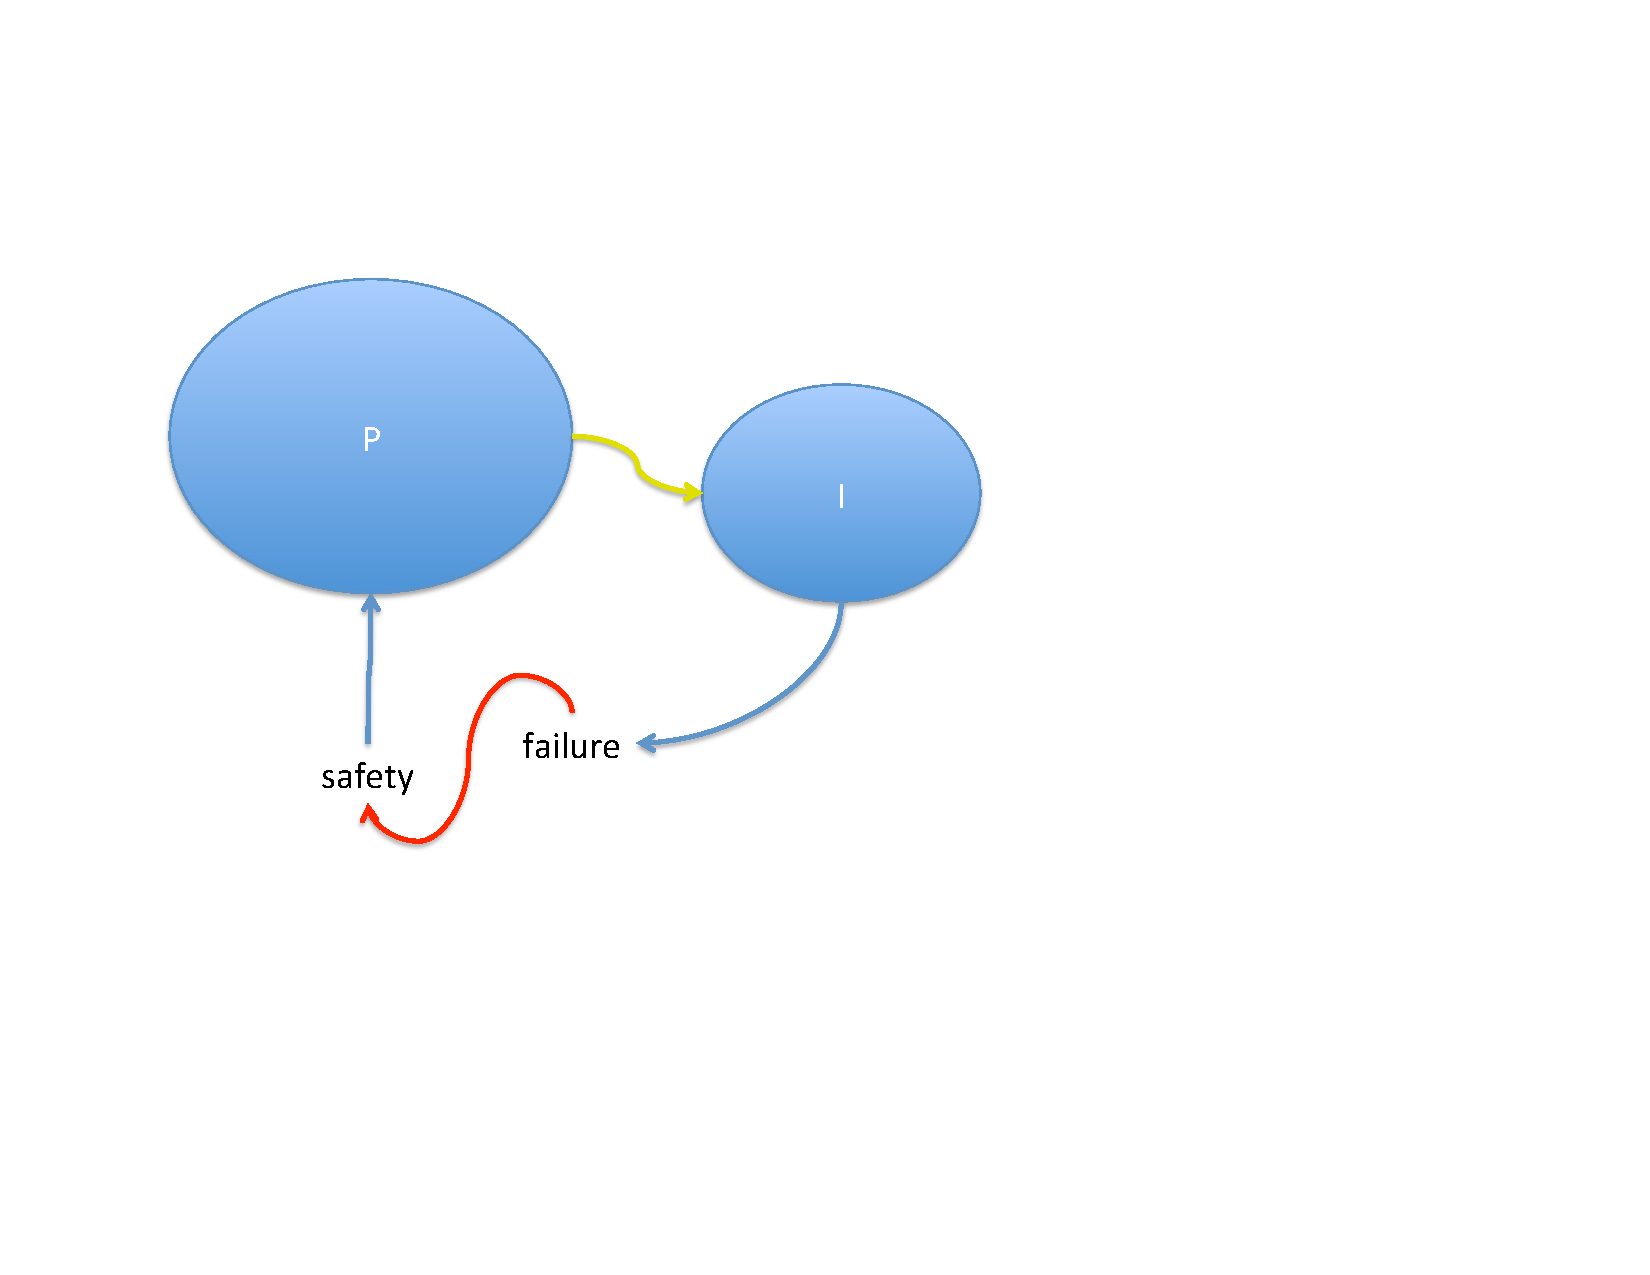
\includegraphics[width=0.9\linewidth]{invariant-rewrite.pdf}
\vspace{-10pt}
\caption{A data dependency graph for a program $P$ and invariants $I$ written in negated form.  $P$ depends positively on \texttt{safety} as shown via a blue arrow, which in turn depends negatively on \texttt{failure}, shown via the red arrow.  In general, the negated $Not_I$ predicates may depend negatively on $P$, hence the yellow arrow.}
\label{fig:invariant-rewrite}
\vspace{-2pt}
\end{figure}

\section{Design Patterns for Coordination Avoidance}
\label{sec:patterns}

\subsection{Design for Commmutativity}
CRDTS, Kohler/Kaashoek.  Works in simple cases, easy to understand.  Recap intro to Neil's paper.
\subsection{Design for Monotonicity}
How can we compose commutative operators?  

\bibliographystyle{abbrv}
\bibliography{safecalm}

\end{document}
